


\section{Automating the Identification of Relevant Text}
\label{cp2:general-approaches}








% many studies have provided possible properties in a natural language artifact
% that guide the automatic identification of relevant text.


In this section, we provide background information on general 
approaches used
by software engineering researchers 
to identify text in natural language software artifacts~\cite{Bavota2016},
where the main goal of such automated approaches is to help
 a person in navigating through the
information patches within an artifact,
thus assisting them in discovering
text that address an information need.
First, we detail concepts 
core to each approach. Then, we 
present seminal work that has applied 
these approaches to problems related 
to software engineering.



% These studies focus on specific tasks such as finding relevant passages in API documentation~\cite{Maalej2013,
% Petrosyan2015, Robillard2015}, learning about API types in code tutorials~\cite{Jiang2016b, Jiang2017},
% or detecting sentences that discuss a bug's expected behaviour~\cite{Chaparro2017}.
% These approaches respectively use the presence of code words, HTML anchor links, or whether a sentence contains
% a modal verb as properties to automatically identify relevant text.



\subsection{Information Retrieval Approaches}


\acf{IR} comprises techniques
or approaches for finding entities (documents, paragraphs, sentences, etc.)
that satisfy an information need~\cite{manning2010IR}.
At its most basic level, 
\acs{IR}
uses the 
frequency or co-occurrence of words (or phrases) to determine the relevance
of an artifact with regards to an information need, often expressed as a query.
We have shown how \acs{IR} identified
books whose subject contained
the keyword `\textit{android}' (Figure~\ref{fig:library-catalogue})
and the same principle could assist 
in finding parts of an artifact that contain some keyword, 
as many web browsers allow via a `\textit{find in page}' feature (Figure~\ref{fig:find-in-page}).







% As an example, Figure~\ref{fig:find-in-page}
% shows that there are 220 matches in a web page 

\medskip
\begin{figure}[h!]
    \centering
    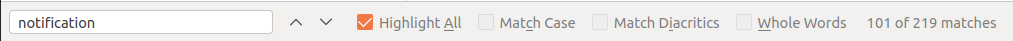
\includegraphics[width=\textwidth]{cp2/find.png}
    \caption{Find in page feature with results for the `\textit{notification}' term}
    \label{fig:find-in-page}
\end{figure}





\acs{IR} identifies and structure all the words, or terms, 
in an artifact so this information can be used for quick access. 
By counting how frequent is a word in 
an artifact and across the entire collection of artifacts, 
one can query which artifacts contain a term and where in the artifact a term appears. 
Using this principle multiple schemes have been proposed 
to identify text based on 
how not all the words in some vocabulary have the same relevance (\textit{TF-IDF})~\cite{luhn1957tf, jones2004idf}, 
how to  represent sentences (\textit{VSM})~\cite{salton1975vector}, 
or how to account for different words that appear in a similar context (\textit{LSI})~\cite{dumais1994latent}.



% Information retrieval applications span several disciplines and it has been used 
% to, for example, assist health workers in searching for medical records~\cite{hanauer2015}
% or to help law practitioners in understanding government regulations~\cite{lau2005legal}.


Information retrieval applications have been used in natural language software artifacts 
as part of approaches that
automatically identify sentences in a bug report that a developer would first read when pressed with time~\cite{Lotufo2012},
or that help cluster software components to aid program comprehension of a software system~\cite{Marcus2003}.



\subsection{Natural Language Processing Approaches}

\acf{NLP} relies on the lexical or syntactical analysis of the text~\cite{jurafsky2014speech}
what might assist in the automatic identification of text that satisfies some information need. 
To illustrate some of the elements obtainable using \acs{NLP}, we consider a short sentence 
instructing how to perform a file system operation using some API: ``\textit{you can use io.StringIO}''.
Figure~\ref{fig:nlp-analysis} shows elements extracted using two \acs{NLP} techniques,
namely \acf{POS} tagging and dependency parsing.
The formed assigns tags  ({\small \textit{PRP}, \textit{VP}, \textit{NNP},} etc.) to each word 
in a sentence~\cite{taylor2003penn}. The latter, identifies
relationships between them, such as how 
`\textit{io.StringIO}' is the direct object (\textit{obj})
associated with the verb `\textit{use}', 
being a potential approach to identify relevant elements in the text.



\medskip
\begin{figure}[h!]
    \centering
    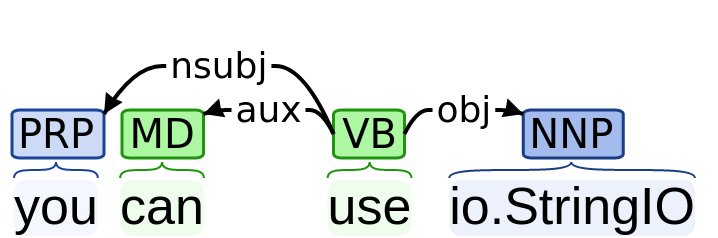
\includegraphics[width=0.40\textwidth]{cp2/textual-analysis.png}
    \caption{Syntactic elements for a sentence giving instructions about how to perform some file system operation}
    \label{fig:nlp-analysis}
\end{figure}


As an example of the application of \ac{NLP} to software engineering text,
Robillard  and Chhetri proposed a tool (Krec)
that uses \acs{POS} tagging to automatically 
identify text with threats and directives on how to use some API element~\cite{Robillard2015}.
As another example, {\small DeMIBuD}
is an automatic approach that uses dependency parsing
to automatically detect sentences discussing a bug's expected behaviour~\cite{Chaparro2017}.






\subsection{Machine Learning Approaches}



Several other studies have investigated regularities in the text 
of natural language artifacts and 
in the meta-data available on them~\cite{Ko2006, Maalej2013, Arya2019}
and a potential way to leverage regularities arising from these empirical studies
is to engineer them into 
features that a  \acf{ML} technique can use to automatically identify or classify
text that is helpful for certain information need~\cite{Bavota2016}. 



Machine learning techniques can be categorized 
in \textit{supervised} or \textit{unsupervised} learning methods 
according to how they make use of available data. 
Supervised learning approaches use a set of features and labeled data
to train classifiers for detecting entities of interest (e.g., text, images, etc.)
while unsupervised learning approaches do not require labeled data and 
identify entities according to properties inferred from the data.



\subsubsection{Supervised Learning Approaches}


With regards to supervised learning approaches, 
we consider the many families of classifiers that 
determine
\textit{(1)} if some entity belongs or not to a given class, as in binary classification
\textit{(2)} which class, out of many, some input entity belongs to, as in multinomial classification, or
\textit{(3)} which classes can be assigned to a given input, as in multi-label classification~\cite{alpaydin2020ml}
and we investigate their application to software engineering problems.





For example, binary classifiers have been used 
to classify text in bug reports that describes (or not) steps to reproduce a bug~\cite{Chaparro2016}
or  to classify paragraphs which contain explanations 
about an API element  in web tutorials~\cite{Petrosyan2015}.
In turn, multinomial classifiers have been mostly used 
to identify a category, out of many, that represents the type of information 
associated with some text. For instance, Arya et al. identified 16 categories of  information available
in open source GitHub issues (e.g., workarounds, solution discussion, task progress, etc.)
and they proposed a multinomial classifier 
to automatically identify such categories~\cite{Arya2019}.
In a similar manner, Fu an colleagues consider 
five types of decisions that might arise during 
email exchanges (e.g., design, testing, management decisions, etc.)
and they proposed a multinomial classifier 
to automatically identify all the decisions present in 
the Hibernate development mailing list~\cite{fu2021}.





Regardless of the type of classifier, these approaches are typically built 
with training data containing human engineered features.
Hence, the cost and effort of hiring skilled workers to produce 
the labeled data for these and other supervised learning approaches
has been a major limitation to their usage in software engineering research~\cite{Arpteg2018, ferreira2021}.




\subsubsection{Unsupervised Learning Approaches}


% Researchers pose the problem of identifying text 
% in a natural language artifact 
% as a binary classification problem. 
% That is, the use of a number of features 
% to predict whether the text is (or not)
% relevant to some context~\cite{aa}.
% In software engineering, 
% binary classifiers have been used for,
% for example, classify text that describes steps to reproduce a bug~\cite{Chaparro2016} or 
% classify text that explains a certain API element, as when 
% Petrosyan et al. used 
%  sentence-level features
% and meta-data features in a classifier 
% that 
% identifies explanations about an API element  in a web tutorial~\cite{Petrosyan2015}.




% Other classification problems predict which class, out of many, some input text belongs to. 
% This type of classification, referred to as multinomial or multi-class classification, 
% is of particular interest if 
% we consider the taxonomies described in Section~\ref{cp2:text-in-se}.
% For example, Arya et al. identified 16 categories of  information available
% in open source GitHub issues (e.g., workarounds, solution discussion, task progress, etc.)~\cite{Arya2019}
% and they proposed a multinomial classifier 
% to automatically identify such categories.








% Although valuable, these classifiers are instances of supervised learning methods.
% They require training data so that a classifier predicts the correct outcome 
% and the cost and effort of hiring skilled workers to produce 
% the labeled data for these and other supervised learning approaches
% has been a major limitation to their usage in software engineering research~\cite{Arpteg2018, ferreira2021}. As an alternative,
% researchers have also explored 
%  unsupervised learning methods---\acs{ML} techniques that do not required training data---for the automatic 
% identification or classification of the text in natural language artifacts~\cite{aa}.





% A common application of unsupervised learning in software engineering
% considers the automatic generation of text summaries.
% Most often, automatic summaries are produced 
% using extractive techniques that select a subset of 
% the sentences of an artifact that will compose the summary~\cite{a}.
% Among other natural language artifacts,
% extractive summarization techniques
% have been applied to Stack Overflow posts~\cite{a}, coding tutorials~\cite{a},
% or bug reports, as
% when Lotufo et al. 
% considered the kinds of sentences a developer would find relevant 
% to understand a bug report when pressed with time~\cite{Lotufo2012},
% and proposed an unsupervised summarization approach 
% based on the PageRank algorithm~\cite{Page1999}
% to identify these sentences. 




% A second set of unsupervised methods focus on clustering data.
% These techniques identify 
% subsets in the data that have similar properties or features 
% and techniques such as \acf{LDA}~\cite{blei2003latent}  have been used both to 
% bootstrap the categorization of information in 
% natural language artifacts and as part of tools that identify 
% portions of the text in an artifact that are helpful to some context. 
% As an example of the former, 
%  Allamanis and Sutton
% applied \acs{LDA}
% to gain insight into the types of questions 
% asked on Stack Overflow~\cite{Allamanis2013}.
% For the latter, tools such as FRAPT
% use \acs{LDA} to identity topics in a web tutorial
% and then extract sentences explaining API elements from each of the topics identified~\cite{Jiang2017}.


% Despite the significant contributions of these and other studies,
% one substantial challenge inherent to the supervised and 
% unsupervised \acs{ML} approaches 
% is that researchers must engineer which 
% features their \acs{ML} technique will use~\cite{ferreira2021}.
% Hence, \acs{ML} approaches have limitations similar to the pattern 
% matching approaches when we consider 
% the specificity and cost of engineering such features
% for a variety of kinds of artifacts.








\subsection{Deep Learning Approaches}






% These studies focus on specific tasks such as finding relevant passages in API documentation~\cite{Maalej2013,
% Petrosyan2015, Robillard2015}, learning about API types in code tutorials~\cite{Jiang2016b, Jiang2017},
% or detecting sentences that discuss a bug's expected behaviour~\cite{Chaparro2017}.
% These approaches respectively use the presence of code words, HTML anchor links, or whether a sentence contains
% a modal verb as properties to automatically identify relevant text.
% Given how quickly developers progress to using new kinds of technology to
% record pertinent information (e.g., slack~\cite{Storey2017, Lin2016}),
% it may be difficult to scale such artifact-centric approaches to cover the range of
% artifacts that could be returned from a search.
% A second issue arises from the fact that coding procedures used to determine relevancy
% in these studies do not consider disagreements~\cite{Stol2015}.
% That is, there are many criteria in how individuals
% assess relevance~\cite{Barry1994, Barry1998, Freund2015}
% and there are no guarantees that
% developers will use the same properties to determine text relevant to their tasks~\cite{Freund2013, Freund2015}.
% In contrast, our study does not pre-assume any relevance cues, and instead,
% we leave the decision of what text is perceived as relevant to a particular task to
% the participants in our experiment.









% Knowledge Recommender ()
% is an example of a
%  tool that uses lexical patterns to 
%  automatically detect relevant text in  API documentation. 
% Krec's premise is that relevant sentences contain a code element, such as a method or class signature.
% These code elements are identifiable via regular expressions 
% and Krec contains a catalog of 361 unique patterns 
% that identify threats and directives on how to use some API element.
% For example, Krec uses the pattern {\small \textit{$\{$may}, \textit{efficient}, \textit{code element regex$\}$}} 
% to identify sentences giving instructions about an efficient way to 
% perform some operation. 



%  is a linguistic-based approach that 

% It uses a set of 154 discourse patterns
% derived from nearly 3,000 bug reports 
% to identify such sentences. 
% For example, the pattern 
% {\small \textit{$\{$subject}, \textit{should/shall (not)}, \textit{complement$\}$}}
% captures common ways with which developers describe a system's expected behaviour
% and empirical assessment of the patterns used by the tool has shown that it 
% detects sentences of interest in bug reports with high accuracy.



% ~\cite{krallinger2017}



% ~\cite{mcdonough2019}